\documentclass[i1]{oss}
\setlength{\topmargin}{-.5in}
\setlength{\textheight}{9in}
\setlength{\oddsidemargin}{.100in}
\setlength{\textwidth}{6.25in}
\usepackage [dutch] {babel}
\usepackage{graphicx}
\usepackage{amsmath}
\usepackage{fullpage}
\usepackage{color}
\usepackage{soul}
\usepackage{gensymb}
\usepackage{caption}
\usepackage{subcaption}
\usepackage[section]{placeins}

\begin{document}

\members{Joren Verspeurt {\small \texttt{(r0258417)} } \\
         Sophie Marien {\small \texttt{(s0216517)}}\\
         Stef Noten {\small \texttt{(s0211264)}}\\
         Toon Nolten {\small \texttt{(r0258654)}} \\
         Begeleider: Mario H. C. T.} % teamleden

\maketitlepage
\newpage
\tableofcontents
\pagebreak




%----------------------------------------------------------------------------------------
%	INLEIDING
%----------------------------------------------------------------------------------------
\section*{Inleiding}
\label{ssec:Inleiding}
%introductie en de belangrijkste elementen van ons ontwerp

Het \emph{JUnit} systeem wordt uitgebreid om een automatische test deamon te maken. Deze uitbreiding wordt uitgevoerd op de achtergrond en moet code van een bepaald project in de gaten houden. Wanneer er code gewijzigt wordt in het project dan zal deamon tests uitvoeren en de ontwikkelaar van deze testen op de hoogte brengen.\\


Voor het ontwerp streven we naar lage coupling. Deamon weet alleen maar af van de actieve policies en de policies waarvoor hem op dat moment de statistieken gaat berekenen. Daemon weet wat hij moet weten en niet te veel. Andere belangrijke klassen zijn \textit{Policy}, \textit{Statistic}, \textit{DataCollector}, \textit{AbstractTestCharacteristics}.


%----------------------------------------------------------------------------------------
%	ONTWERP
%----------------------------------------------------------------------------------------
\section{Ontwerp}
\label{ssec:Ontwerp}
%Klassendiagram en interactie diagrammen

In deze sectie bespreken we het algemene ontwerp en de ontwerpbeslissingen. In de eerste subsectie wordt het klassendiagram besproken samen met een aantal verschillen met het vorige klassendiagram.
In de tweede sectie worden de interactiediagrammas besproken die 

%-------------KLASSENDIAGRAMMA-------------------------------
\subsection{Klassendiagramma}
\label{ssec:Klassendiagramma}

Elke klassen heeft zijn eigen specifieke verantwoordelijkheid:

\begin{description}

\item \textit{Deamon}: \textit{Deamon} is verantwoordelijk voor het opstarten van de TestRuns. Het is alleen maar vanop de hoogte van de active policies.

\item \textit{SortingPolicy}:\textit{SortingPolicy} is verantwoordelijk voor het ordenen van de testen volgens een bepaalde policy en voor het filteren van de testen.

\item \textit{Statistic}: \textit{Statistic} is verantwoordelijk voor het berekenen van de statistieken.

\item \textit{StatisticManager}:

\item \textit{DataCollector}: \textit{DAtaCollector} heeft de verantwoordelijkheid om gegenereerde data te laten horen bij een description van een testcase in plaats van testklassen en suites. 

\item \textit{DataCollectorManager}:

\item \textit{AbstractTestCharacteristic}:



\end{description}


%figuur oud klassendiagram
\begin{figure}[tbp]
\begin{center}
    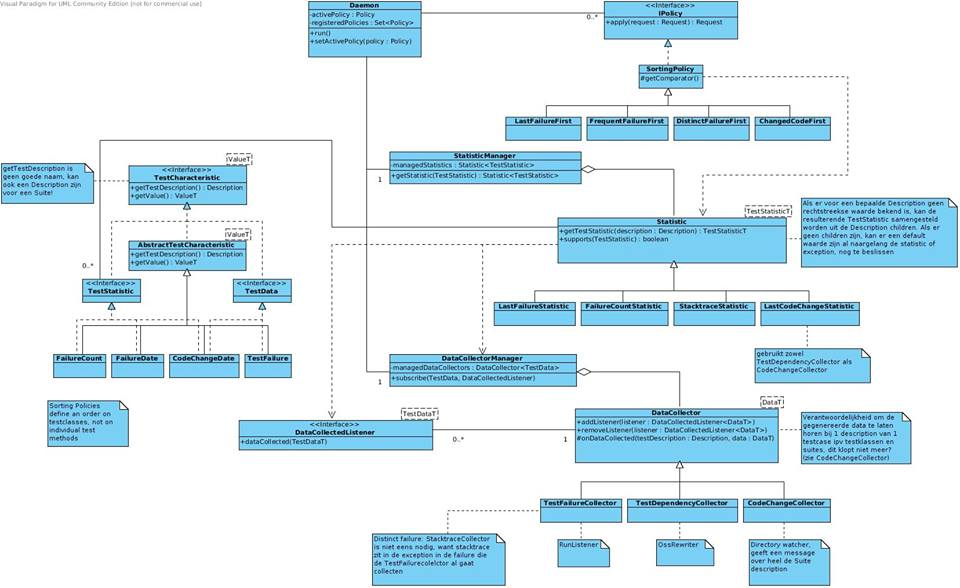
\includegraphics[width=0.8\textwidth]{klassendiagramOud}
    \caption{Grafische User Interface}
	\label{fig:gui}
\end{center}
\end{figure}



%figuur nieuw klassendiagram
\begin{figure}[tbp]
\begin{center}
    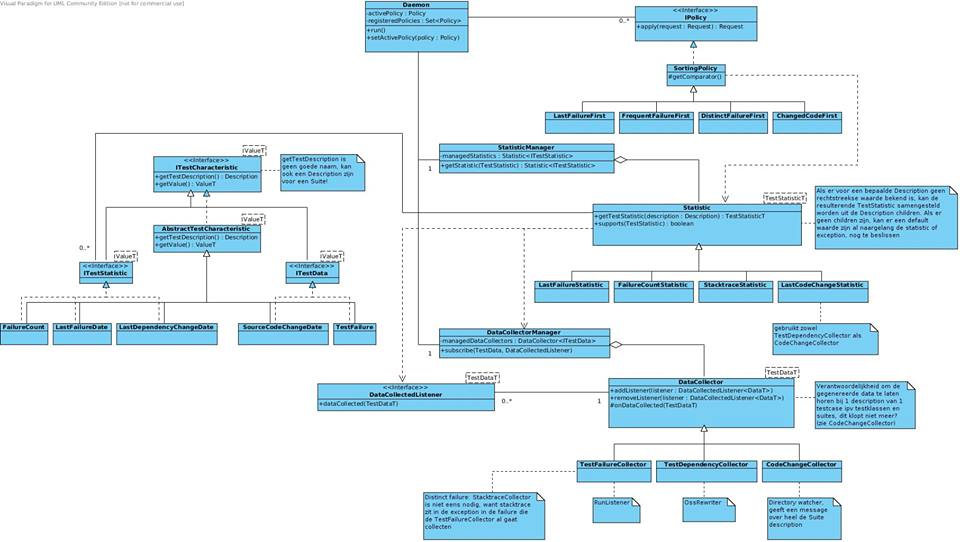
\includegraphics[width=0.8\textwidth]{klassendiagram}
    \caption{Grafische User Interface}
	\label{fig:gui}
\end{center}
\end{figure}

%-------------Interactie Diagrammas-------------------------------
\subsection{Interactie diagrammas}
\label{ssec:Interactiedia}







%-------------Ontwerpbeslissingen-------------------------------
\subsection{Ontwerpbeslissingen en patronen}
\label{ssec:Ontwerpbeslissingen}

Helemaal in het begin werd er geopteerd voor het Model-View-Controller Pattern. Hierbij zou de view de \textit{GUI}, \textit{CLI} zijn. De Controller zou een input besturingsview zijn die input en output handelde en als laatste de Model zouden de verschillende klassen zijn: \textit{Daemon, Policy, TestInfomation, DataCollector, Statistic, TestRun}. \\

Hiervan werd er toch afgestapt om het ontwerp anders te implementeren. \\
%TODO waarom?


\begin{description}
\item Statistieken verzamelen. (Het verwerpen van de statistic pool)
In het begin was er in het ontwerp een \textit{Statistic Pool}. Deze pool zou de statistieken bijhouden. Hier wordt dan aan opgevraagd of er een specifiek statistiek in zit. Is dit niet zo dan wordt deze geregistreerd. Deze werd uiteindelijk toch verworpen want er zou teveel afhangen van deze klasse. Er worden nog steeds statistieken bijgehouden maar dit wordt gedaan in \textit{StatisticManager}.
%TODO is dit correct?

\item Policies
Samengestelde filters en sorting policies
We hebben een Policy die een apply, die op een request werkt en een request teruggeeft. Daarnaast hebben we dat elke Policy een child Policy heeft. Als de apply aangeroepen wordt, wordt eerst de apply van de child opgeroepen en daarna zijn eigen apply op het resulterende request. Hiervoor kunnen we niet garanderen dat het resultaat correct volgens meerdere sorteringen gedaan wordt. SortingRequest kan dit niet over meerdere niveaus heen (stel dat er een filterRequest tussenzit). Naar buiten toe is de aanname dus is dat de nieuwe sortering de vorige sortering teniet kan doen ipv samenstellen.
%TODO dit was veranderd naar een ander ontwerp

\item Collectors
Voor FailureTraceColelctor zijn de parallelle testen niet ondersteund. Dit wordt gedaan omdat het op dit moment teveel werk is om te onderscheiden welke methode-oproepen van welke test komen.
\end{description}



%

%----------------------------------------------------------------------------------------
%	TESTEN
%----------------------------------------------------------------------------------------
\section{Testen}
\label{ssec:testen}
%Een hoofdstuk rond testen dat de procedure beschrijft die gevolgd werd bij het testen: wat
%werd getest en hoe?


%----------------------------------------------------------------------------------------
%	PROJECT MANAGMENT
%----------------------------------------------------------------------------------------
\section{Project management}
\label{ssec:Projectmanag}
%taakverdeling elk lid en welke taak
%uren

%TODO tekst

%TODO laatste week aanvullen!!
\begin{table}[h!]
\begin{center}
    \begin{tabular}{ r | c  c  c  c  c  c}
     & Joren & Toon & Stef & Sophie \\ \hline
    Algemeen & 2u00 & 2u00 & 2u00 & 2u00\\
           Tools & 8u30 & 8u30 & 8u00 & 4u30 \\
        Analyse & 10u00 & 10u00 & 12u15 & 12u00 \\
        Ontwerp & 00u00 & 00u00 & 00u00 & 00u00 \\
        Implementeren & 00u00 & 00u00 & 00u00 & 00u00\\
        Verslag & 9u00 & 9u00 & 9u00 & 9u00 \\
        Totaal & 29u30 & 29u30 & 31u15 & 27u30  
    \end{tabular}
    \caption{Overzicht werkuren per onderdeel}
    \label{tab:werkuren}
\end{center}
\end{table}

%TODO figuren updaten
\begin{figure}[h!]
        \centering
        \begin{subfigure}[hb]{0.20\textwidth}
                \centering
                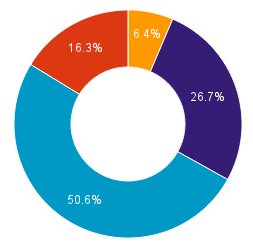
\includegraphics[width=\textwidth]{chart_2}
                \caption{Joren}
        \end{subfigure}%
        \begin{subfigure}[hb]{0.20\textwidth}
                \centering
                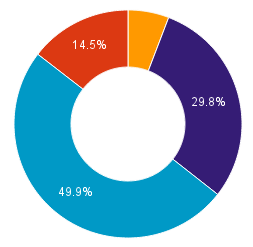
\includegraphics[width=\textwidth]{chart_3}
                \caption{Toon}
        \end{subfigure}%
        \begin{subfigure}[hb]{0.20\textwidth}
                \centering
                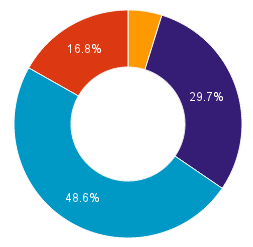
\includegraphics[width=\textwidth]{chart_4}
                \caption{Stef}
        \end{subfigure}%
        \begin{subfigure}[hb]{0.20\textwidth}
                \centering
                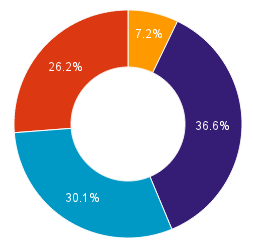
\includegraphics[width=\textwidth]{chart_5}
                \caption{Sophie}
        \end{subfigure}%
                \begin{subfigure}[hb]{0.20\textwidth}
                \centering
                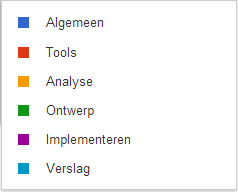
\includegraphics[width=\textwidth]{legende}
                \caption{Legende}
        \end{subfigure}%


 \caption{Weergave van de werkverdeling}
\label{fig:werkverdeling}
\end{figure}





%----------------------------------------------------------------------------------------
%	 CONCLUSIE en DISCUSSIE
%----------------------------------------------------------------------------------------
\section{Conclusie}
\label{ssec:Conclusie}
% Een hoofdstuk met een discussie en conclusie waarin interessante ervaringen, problemen en
%andere opmerkingen omtrent het project worden beschreven



%----------------------------------------------------------------------------------------
%	GLOSSARY
%----------------------------------------------------------------------------------------
\section{Glossary}
\label{ssec:glossary}


Daemon met een policy en een testinformation Klasse en een Statistic information 

Pattern Model-View-Controller
View:  GUI, CLI, passive view
Controller:
Input besturingsview, handeld input/output
Model: Daemon, Policy, TestInfomation, DataCollector, Statistic, TestRun
Daemon is bedoeld als interface voor het model

Verantwoordelijkheden
Policy: ordening, filtering
Statistic: berekent de statistieken, legt een strategie vast om data op te vragen.
TestInformation:  Houdt de statistieken bij (alles dat uit de collectors wordt opgevraagd)
DataCollector: Data verzameling, inpluggen in een TestRun, change code bijhouden (apart in een andere Collector)
Daemon:  Starten van TestRuns
TestRun:  runnen van testen

Implementaties:
Policy als Composit/Decorator/Strategy
We weten niet zeker of het een composit is want er werd getwijfeld tussen Composit en Decorator Pattern. 
Statistic en DataCollector zijn een Strategy
TestInfomation
Eerst mapte Description met een lijst van tuples. Dit is veranderd naar TestSummary
Map<Description,OrderedSet<TestSummary>>
	TestSummary	-Map<Collector, Object>
			- TestID


We streven voor low-coupling. 

Verslag: beginnen met de analyse van wat we nodig hebben en daarna uitleggen hoe we dit oplossen en analyseren en bediscussiëren.

 


\end{document}



